\documentclass[a4paper,11pt,draft]{article}

\usepackage[finnish]{babel}
\usepackage[utf8]{inputenc}
\usepackage[margin=2cm]{geometry}
\usepackage{amsfonts,amsmath,amssymb,amsthm,enumitem}
\usepackage{pgf}
\usepackage{tikz}
\usetikzlibrary{arrows,automata}

\newtheorem*{claim}{Väite}

\newcommand{\set}[1]{{\left\{ #1 \right\}}}
\newcommand{\ceil}[1]{{\left\lceil#1\right\rceil}}
\newcommand{\stateseq}[5]{{%
\begin{automata}[1.3]
      \tikzstyle{every state}=[fill=none,draw=none,text=black,minimum
        size=0.8cm,inner sep=0cm]
      \node[state]                     (r1)                   {$#2_1$};
      \node[state,node distance=#5]    (r2)   [right of=r1]   {$#2_2$};
      \node[state]                     (dots) [right of=r2]   {$\ldots$};
      \node[state]                     (rn)   [right of=dots] {$#2_{n+1}$};
      \node[state,node distance=0.5cm] (sa)   [below of=r1]   {$#3$};
      \node[state,node distance=0.5cm] (dsa)  [below of=r2]   {$#4$};

        \path (r1)   edge [bend left=20] node {$#1_1$} (r2)
              (r2)   edge [bend left] node {$#1_2$} (dots)
              (dots) edge [bend left] node {$#1_n$} (rn);
    \end{automata}%
}}

\newenvironment{automata}[1][2.8]%
{\begin{tikzpicture}[->,>=stealth',shorten >=1pt,auto,node distance=#1cm,semithick]}%
{\end{tikzpicture}}

\begin{document}

\subsection*{582206 Laskennan mallit, syksy 2012 \\
  \textmd{3. harjoitusten malliratkaisut \\
    Juhana Laurinharju ja Jani Rahkola}}

\begin{enumerate}
\item
  Olkoon $N_1$ ja $N_2$ epädeterministiset automaatit jotka on kuvattu
  alla. Tunnistavatko automaatit seuraavat sanat?

  \begin{center}
    \begin{tabular}{cc}
      \begin{tabular}{l|c|c}
        & $N_1$ & $N_2$ \\
        \hline
        $a$ & kyllä & ei \\
        $aa$ & kyllä & ei \\
        $aab$ & ei & ei \\
        $\varepsilon$ & kyllä & kyllä \\
        $ab$ & ei & kyllä \\
        $abab$ & ei & kyllä \\
        $aba$ & ei & kyllä \\
        $abaa$ & ei & ei
      \end{tabular}
      &
      \begin{tabular}{cc}
        $N_1$: & $N_2$: \\
        \begin{automata}[2]
          \node[state,initial above,accepting] (q0)               {$q_0$};
          \node[state]                         (q1) [below of=q0] {$q_1$};
          
          \path (q0) edge [loop right] node {$a$} ()
          edge              node {$a$} (q1)
          (q1) edge [loop right] node {$b$} ();
        \end{automata}
        &
        \begin{automata}[2]
          \node[state,initial,accepting] (q0)               {$q_0$};
          \node[state]                   (q1) [right of=q0] {$q_1$};
          \node[state,accepting]         (q2) [right of=q1] {$q_2$};
          \node[state,accepting]         (q3) [below of=q1] {$q_3$};
          
          \path (q0) edge             node        {$a$} (q1)
          (q1) edge             node        {$b$} (q2)
          edge             node        {$b$} (q3)
          (q2) edge [bend left] node        {$a$} (q1)
          (q3) edge             node [swap] {$a$} (q2);
        \end{automata}
      \end{tabular}
    \end{tabular}
  \end{center}

\item
  Minkälaisia sanoja seuraavat äärelliset epädeterministiset
  automaatit hyväksyvät?
  \begin{enumerate}
  \item \hfill \\
    \begin{automata}[2]
      \node[state,initial,accepting] (q0)               {$q_0$};
      \node[state]                   (q1) [right of=q0] {$q_1$};
      \node[state] (q2) [below of=q0] {$q_2$};

      \path (q0) edge [loop above] node {$a$}   ()
                 edge              node [swap]{$b$}  (q1)
            (q1) edge              node {$a$}  (q2)
            (q2) edge              node {$a$} (q0);
    \end{automata}

    Jokaisen $b$:n jälkeen on ainakin kaksi $a$:ta. Automaatin määrittelemä
    säännöllinen kieli on siis $(\set{a} \cup \set{baa})^*$ joka voidaan
    kuvata myös säännöllisellä lausekkeella $(a | baa)^*$.

  \item \hfill \\
    \begin{automata}[2]
      \node[state,initial]   (q0)               {$q_0$};
      \node[state]           (q1) [right of=q0] {$q_1$};
      \node[state]           (q2) [right of=q1] {$q_2$};
      \node[state,accepting] (q3) [right of=q2] {$q_3$};

      \path (q0) edge               node      {$a$}   (q1)
            (q1) edge               node       {$a$}  (q2)
            (q2) edge               node       {$a$} (q3)
                 edge  [bend right] node [swap]{$a$} (q0)
            (q3) edge  [bend left]  node       {$a$} (q0);
    \end{automata}

    Rakennetaan automaattia vastaava deterministinen automaatti.

    \begin{automata}[2.5]
      \tikzstyle{every state}=[shape=rectangle,rounded corners];
      \node[initial below,state] (q0)                   {$\set{q_0}$};
      \node[state]           (q1)     [right of=q0] {$\set{q_1}$};
      \node[state]           (q2)     [right of=q1] {$\set{q_2}$};
      \node[accepting,state] (q03)    [right of=q2] {$\set{q_0,q_3}$};
      \node[state]           (q01)    [below of=q03] {$\set{q_0,q_1}$};
      \node[state]           (q12)    [left of=q01] {$\set{q_1,q_2}$};
      \node[state]           (q02)    [left of=q12] {$\set{q_0,q_2}$};
      \node[accepting,state] (q013)   [left of=q02] {$\set{q_0,q_1,q_3}$};
      \node[state]           (q012)   [left of=q013] {$\set{q_0,q_1,q_2}$};
      \node[accepting,state] (q0123) [above of=q012] {$\set{q_9,q_1,q_2,q_3}$};

      \node[accepting,state] (q3)     [above of=q0] {$\set{q_3}$};
      \node[state]           (qe)     [left of=q3] {$\emptyset$};
      \node[accepting,state] (q13)    [below of=q02] {$\set{q_1,q_3}$};
      \node[accepting,state] (q23)    [above of=q03] {$\set{q_2,q_3}$};
      \node[accepting,state] (q023)   [below of=q013] {$\set{q_0,q_2,q_3}$};
      \node[accepting,state] (q123)   [below of=q023] {$\set{q_1,q_2,q_3}$};

      \path (q0)   edge node {$a$} (q1)
            (q1)   edge node {$a$} (q2)
            (q2)   edge node {$a$} (q03)
            (q03)  edge node {$a$} (q01)
            (q01)  edge node {$a$} (q12)
            (q12)  edge node {$a$} (q02)
            (q02)  edge node {$a$} (q013)
            (q013) edge node {$a$} (q012)
            (q012) edge node {$a$} (q0123)
            (q3)   edge node {$a$} (q0)
            (q23)  edge node {$a$} (q03)
            (q13)  edge node {$a$} (q02)
            (q023) edge node {$a$} (q013)
            (q123) edge node {$a$} (q023);
    \end{automata}

    Deterministisestä automaatista voidaan huomata, että automaatti hyväksyy
    kaikki merkkijonot, joissa on kolme, kuusi, seitsemän tai vähintään
    yhdeksän $a$:ta.

    Säännöllisenä lausekkeena kielen voi kirjoittaa esimerkiksi
    $aaa(aaa|aaaa)^*$ (muodostettu vastaamaan epädeterminististä automaattia)
    tai $(a^3|a^6|a^7|a^9a^*)$ (muodostettu deterministisen automaatin
    antamasta lukumääräintuitiosta)
  \end{enumerate}

\item
  Piirrä epädeterministiset automaatit tiloineen ja siirtymänuolineen
  seuraaville kielille.
  \begin{enumerate}
  \item
    $L = \set{w \in \set{a, b}^* \mid \mbox{$w$ sisältää korkeintaan
      kaksi $a$:ta}}$
  \item
    $L = \set{w \in \set{a, b}^* \mid \mbox{$w$ sisältää parillisen
      määrän alimerkkijonoa $ab$}}$
  \item
    $L = \set{w \in \set{a,b}^* \mid \mbox{$w$:n ensimmäinen ja
      viimeinen kirjain ovat samat}}$
  \end{enumerate}

  \begin{enumerate}
    \item \mbox{}

      \begin{center}
        \begin{automata}[2.2]
          \node[initial, state, accepting] (q1)               {$q_1$};
          \node[state, accepting]          (q2) [right of=q1] {$q_2$};
          \node[state, accepting]          (q3) [right of=q2] {$q_3$};

          \path (q1) edge node {$a$} (q2)
          (q2) edge node {$a$}(q3)

          (q1) edge [loop above] node {$b$} (q1)
          (q2) edge [loop above] node {$b$} (q2)
          (q3) edge [loop above] node {$b$} (q3);
        \end{automata}
      \end{center}

    \item \mbox{}

      \begin{center}
        \begin{automata}[2.2]
          \node[initial, accepting, state] (q0)               {$q_0$};
          \node[accepting, state]          (q1) [right of=q0] {$q_1$};
          \node[state]                     (q2) [right of=q1] {$q_2$};
          \node[state]                     (q3) [right of=q2] {$q_3$};

          \path (q0) edge [loop above] node {$b$} (q0)
          (q1) edge [loop above] node {$a$} (q1)
          (q2) edge [loop above] node {$b$} (q2)
          (q3) edge [loop above] node {$a$} (q3)

          (q0) edge node {$a$} (q1)
          (q1) edge node {$b$} (q2)
          (q2) edge node {$a$} (q3)
          (q3) edge [bend left] node {$b$} (q0) ;
        \end{automata}
      \end{center}

    \item \mbox{}

      \begin{center}
        \begin{automata}[2.2]
          \node[initial, state]   (q0)                            {$q_0$};
          \node[state, accepting] (q1) [right of=q0]              {$q_1$};
          \node[state]            (q2) [right of=q0, above of=q0] {$q_2$};
          \node[state]            (q3) [right of=q0, below of=q0] {$q_3$};
          \node[state, accepting] (q4) [right of=q2]              {$q_4$};
          \node[state, accepting] (q5) [right of=q3]              {$q_5$};

          \path (q0) edge              node {$a,b$} (q1)
          (q0) edge              node {$a$}   (q2)
          (q0) edge              node {$b$}   (q3)
          (q2) edge [loop above] node {$a,b$} (q2)
          (q2) edge              node {$a$}   (q4)
          (q3) edge [loop below] node {$a,b$} (q3)
          (q3) edge              node {$b$}   (q5);
        \end{automata}
      \end{center}
  \end{enumerate}

\item
  Merkkinon $w=w_1 w_2 \dots w_n$ \textit{käänteismerkkijono} on
  $w^{{\cal R}}=w_n w_{n-1}\dots w_1$. Olkoon kielen $A$
  \textit{käänteiskieli} $A^{{\cal R}} = \set{w^{{\cal R}}\mid w \in
    A}$. Näytä että jos $A$ on säännöllinen niin myös $A^{{\cal R}}$
  on sään\-nöl\-li\-nen (vihje: käytä epädeterministisyyttä apuna). Tee myös
  pienet esimerkit.

  Muodostetaan ensin pari esimerkkiä. Tässä automaatti, joka tunnistaa kaikki
  merkkijonot, jotka alkavat joko $aab$:llä tai $bba$:lla.

  \begin{center}
    \begin{automata}[2.2]
      \node[initial, state] (q0)                          {$q_0$};
      \node[state]        (q1) [right of=q0]{$q_1$};
      \node[state]        (q2) [right of=q0, above of=q0] {$q_2$};
      \node[state]        (q3) [right of=q2]              {$q_3$};
      \node[state]        (q4) [right of=q0, below of=q0] {$q_4$};
      \node[state]        (q5) [right of=q4]              {$q_5$};
      \node[accepting,state]   (q6) [right of=q3, below of=q3] {$q_6$};

      \path (q0) edge node {$a$} (q2)
      (q0) edge node {$b$} (q4)
      (q4) edge node {$b$} (q5)
      (q2) edge node {$a$} (q3)
      (q3) edge node {$b$} (q6)
      (q5) edge node {$a$} (q6)

      (q2) edge node {$b$} (q1)
      (q4) edge node {$a$} (q1)
      (q3) edge node {$a$} (q1)
      (q5) edge node {$b$} (q1)

      (q6) edge [loop right] node {$a,b$} (q6)
      (q1) edge [loop right] node {$a,b$} (q1) ;
    \end{automata}
  \end{center}

  Tälle voidaan nyt helposti muodostaa käänteiskielen automaatti asettamalla
  lopputila alkutilaksi, alkutila lopputilaksi ja kääntämällä kaikki nuolet
  ympäri.

  \begin{center}
    \begin{automata}[2.2]
      \node[accepting, state] (q0)                          {$q_0$};
      \node[state]        (q1) [right of=q0]{$q_1$};
      \node[state]        (q2) [right of=q0, above of=q0] {$q_2$};
      \node[state]        (q3) [right of=q2]              {$q_3$};
      \node[state]        (q4) [right of=q0, below of=q0] {$q_4$};
      \node[state]        (q5) [right of=q4]              {$q_5$};
      \node[initial above,state]   (q6) [right of=q3, below of=q3] {$q_6$};

      \path (q2) edge node {$a$} (q0)
      (q4) edge node {$b$} (q0)
      (q5) edge node {$b$} (q4)
      (q3) edge node {$a$} (q2)
      (q6) edge node {$b$} (q3)
      (q6) edge node {$a$} (q5)

      (q1) edge node {$b$} (q2)
      (q1) edge node {$a$} (q4)
      (q1) edge node {$a$} (q3)
      (q1) edge node {$b$} (q5)

      (q6) edge [loop right] node {$a,b$} (q6)
      (q1) edge [loop right] node {$a,b$} (q1) ;
    \end{automata} 
  \end{center}

  Ja näin saatiin epädeterministinen automaatti, joka tunnistaa kaikki
  merkkijonot jotka loppuvat joko $baa$ tai $abb$.

  Alkuperäinen automaatti oltaisiin kuitenkin voitu muodostaa myös
  seuraavasti:

  \begin{center}
    \begin{automata}[2.2]
      \node[initial, state] (q0)                          {$q_0$};
      \node[state]        (q1) [right of=q0]{$q_1$};
      \node[state]        (q2) [right of=q0, above of=q0] {$q_2$};
      \node[state]        (q3) [right of=q2]              {$q_3$};
      \node[state]        (q4) [right of=q0, below of=q0] {$q_4$};
      \node[state]        (q5) [right of=q4]              {$q_5$};
      \node[accepting,state]   (q6) [right of=q5] {$q_6$};
      \node[accepting,state]   (q7) [right of=q3] {$q_7$};

      \path (q0) edge node {$a$} (q2)
      (q0) edge node {$b$} (q4)
      (q4) edge node {$b$} (q5)
      (q2) edge node {$a$} (q3)
      (q3) edge node {$b$} (q7)
      (q5) edge node {$a$} (q6)

      (q2) edge node {$b$} (q1)
      (q4) edge node {$a$} (q1)
      (q3) edge node {$a$} (q1)
      (q5) edge node {$b$} (q1)

      (q6) edge [loop below] node {$a,b$} (q6)
      (q7) edge [loop above] node {$a,b$} (q7)
      (q1) edge [loop right] node {$a,b$} (q1) ;
    \end{automata}
  \end{center}

  Nyt voidaan huomata, että automaattia kääntäessä tarvittaisiin kaksi
  aloitustilaa, sillä alkuperäisessä automaatissa on useampia hyväksyviä
  tiloja.

  Ongelma voidaan korjata lisäämällä käänteiskielen automaattiin uusi
  aloitustilan, josta tulee $\varepsilon$-siirtymät jokaiseen haluttuun
  aloitustilaan.

  \begin{center}
    \begin{automata}[2.2]
      \node[accepting, state] (q0)                          {$q_0$};
      \node[state]        (q1) [right of=q0]{$q_1$};
      \node[state]        (q2) [right of=q0, above of=q0] {$q_2$};
      \node[state]        (q3) [right of=q2]              {$q_3$};
      \node[state]        (q4) [right of=q0, below of=q0] {$q_4$};
      \node[state]        (q5) [right of=q4]              {$q_5$};
      \node[state]   (q6) [right of=q5] {$q_6$};
      \node[state]   (q7) [right of=q3] {$q_7$};
      \node[state, initial right] (q8) [right of=q7, below of=q7] {$x$};

      \path (q2) edge node {$a$} (q0)
      (q4) edge node {$b$} (q0)
      (q5) edge node {$b$} (q4)
      (q3) edge node {$a$} (q2)
      (q7) edge node {$b$} (q3)
      (q6) edge node {$a$} (q5)

      (q1) edge node {$b$} (q2)
      (q1) edge node {$a$} (q4)
      (q1) edge node {$a$} (q3)
      (q1) edge node {$b$} (q5)

      (q7) edge [loop above] node {$a,b$} (q7)
      (q6) edge [loop below] node {$a,b$} (q6)
      (q1) edge [loop right] node {$a,b$} (q1) 

      (q8) edge node {$\varepsilon$} (q7)
      (q8) edge node {$\varepsilon$} (q6);

    \end{automata}
  \end{center}

  Kun nyt ollaan saatu intuitio siitä miten kääntäminen pitäisi tehdä,
  voidaan tämä vielä kirjoittaa formaalisti.

  Olkoon $M = (Q,\Sigma,\delta,s,F)$ kielen $A$ tunnistava deterministinen
  automaatti. Muodostetaan nyt yllä olevien esimerkkien motivoimana
  epädeterministinen automaatti $M^\mathcal{R}$ käänteiskielelle
  $A^\mathcal{R}$.

  \begin{align*}
    Q^\mathcal{R} &= Q \cup \set{x}\textrm{, missä } \notin Q
                  & \textrm{uusi alkutila} \\
    \Sigma^\mathcal{R} &= \Sigma \cup \set{\epsilon}
                  & M^\mathcal{R} \textrm{ epädeterministinen} \\
    \delta^\mathcal{R}(q_i, \sigma)
                  &= \set{q_j \in Q \mid \delta(q_j, \sigma) = q_i}
                  & \textrm{kaikki $M$:n tilat, joista pääsee}
                  \textrm{ $\sigma$:lla nykyiseen tilaan}\\
    \delta^\mathcal{R}(x,\epsilon) &= F
                  & \textrm{uudesta alkutilasta pääsee suoraan}
                    \textrm{ $M$:n kaikkiin lopputiloihin} \\
    \delta^\mathcal{R}(x, \sigma) &= \emptyset
                  & \textrm{uudesta alkutilasta ei ole siirtymiä $\Sigma$:n }
                    \textrm{merkeillä} \\
    F^\mathcal{R} &= \set{s} & M^\mathcal{R} \textrm{:n ainoa hyväksyvä tila }
                  \textrm{on $M$:n alkutila}
  \end{align*}

  Nyt ollaan siis muodostettu automaatti, joka aloittaa alkuperäisen
  automaatin hyväksyvistä tiloista, lopettaa alkuperäisen automaatin
  alkutilaan ja kääntää kaikki nuolet ympäri.

\item
  Muunna seuraavat epädeterministiset automaatit deterministisiksi
  käyttämällä lauseen 1.39 todistusta apuna.

  \begin{tabular}{cc}
    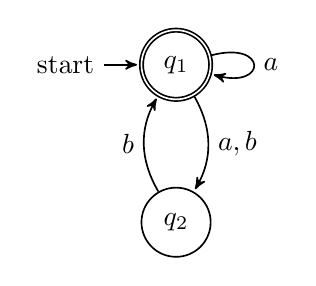
\begin{tikzpicture}[->,>=stealth',shorten >=1pt,auto,node distance=2cm,semithick]

      \node[state,initial,accepting] (q1)               {$q_1$};
      \node[state]                   (q2) [below of=q1] {$q_2$};

      \path (q1) edge [loop right]  node      {$a$}   ()
      edge  [bend left]       node     {$a,b$}  (q2)
      (q2) edge  [bend left]       node       {$b$}  (q1);
    \end{tikzpicture} 
    & 
    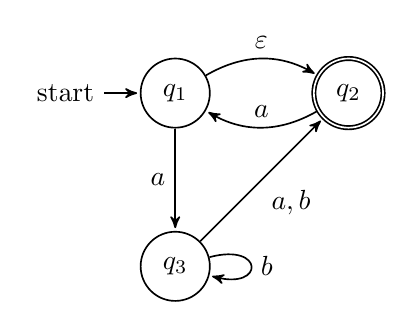
\begin{tikzpicture}[->,>=stealth',shorten >=1pt,auto,node distance=2.2cm,semithick]

      \node[state,initial]	(q1)  				{$q_1$};
      \node[state,accepting]	(q2) [right of=q1] {$q_2$};
      \node[state]   		(q3) [below of=q1] {$q_3$};
      
      \path (q1) edge   				node [swap]	{$a$}  	(q3)
      edge [bend left] 	node 		{$\varepsilon$} 	(q2)
      (q2)	edge [bend left]	node [swap]   	{$a$}	(q1)       
      (q3) edge				node [swap]	{$a,b$}	(q2)
      edge [loop right]   node    {$b$} ();        
    \end{tikzpicture}
    \\
    \begin{automata}[2.5]
          \tikzstyle{every state}=[shape=rectangle,rounded corners];
          \node[accepting, initial above, state] (q1) {$\set{q_1}$};
          \node[state]       (q2)  [below of=q1, left of=q1] {$\set{q_2}$};
          \node[state]       (q)   [above of=q2] {$\emptyset$};
          \node[accepting, state] (q12) [below of=q1] {$\set{q_1,q_2}$};
    
          \path (q1)  edge              node {$a$}   (q12)
                (q1)  edge [bend left=10]  node {$b$}   (q2)
                (q2)  edge              node {$a$}   (q)
                (q2)  edge [bend left=10]  node {$b$}   (q1)
                (q)   edge [loop above] node {$a,b$} (q)
                (q12) edge [loop right] node {$a,b$} (q12);
    \end{automata}
    &
    \begin{automata}
      \tikzstyle{every state}=[shape=rectangle,rounded corners];
      \node[initial above, accepting, state] (q12) {$\set{q_1,q_2}$};
      \node[accepting, state] (q123) [right of=q12]
           {$\set{q_1,q_2,q_3}$};
      \node[state] (q) [below of=q12]{$\emptyset$};
      \node[state] (q23) [right of=q123]{$\set{q_2,q_3}$};

      \path (q12)  edge              node {$a$}   (q123)
            (q12)  edge              node {$b$}   (q)
            (q)    edge [loop right] node {$a,b$} (q)
            (q123) edge [loop above] node {$a$}   (q123)
            (q123) edge              node {$b$}   (q23)
            (q23)  edge [loop above] node {$b$}   (q23)
            (q23)  edge [bend left]  node {$a$}   (q12) ;
    \end{automata}
  \end{tabular}

\item 
  Olkoon $M$ \textbf{deterministinen} automaatti, missä on $n$ tilaan,
  ja $L(M)=A$. (vihje ajattele syklejä)
  \begin{enumerate}
  \item
    \begin{claim}
      Todista että $A\neq \emptyset \Leftrightarrow \exists w \in A$
      mille $|w| < n$.
    \end{claim}
    \begin{proof}
      \hfill \\
      \begin{description}
        \item[``$\Leftarrow$''] \hfill \\
          Koska on olemassa $w \in A$, ei $A$ ole tyhjä.
        \item[``$\Rightarrow$''] \hfill \\
          Lähdetään osoittamaan väitettä seuraavasti:
          \begin{itemize}
            \item
              Otetaan merkkijono $w \in A, w = w_1w_2 \ldots w_k$
            \item
              Tarkastellaan tilajonoa $\bar{q} = q_1q_2 \ldots
              q_{k+1}$ jonka läpi automaatti $M$ kulkee merkkijonolla
              $w$.
            \item
              Poistetaan tilajonosta $\bar{q}$ kaikki mahdollisesti
              löytyvät silmukat.
            \item
              Edellisen kohdan tuloksena saatua tilajonoa vastaa jokin
              merkkijono $u \in A$ jolla on haluttu ominaisuus.
          \end{itemize}
          Koska $A \neq \emptyset$, niin löytyy $w \in A, w = w_1w_2
          \ldots w_k$, ja olkoon $M = (Q, \Sigma, \delta, s, F)$.
          Määritellään tilajono $\bar{q} = q_1q_2 \ldots q_{k+1}$
          missä $q_1 = s$ ja $q_{i+1} = \delta(q_i, w_i)$.
          \begin{center}
            \stateseq{w}{q}{s}{\delta(s, u_1)}{1.5cm}
          \end{center}
          \begin{enumerate}
          \item
            Jos $|w| < n$, niin $u$ on etsitty merkkijono.
          \item
            Jos $|w| \ge n$, niin lokeroperiaatteen nojalla löytyy
            $q_i = q_j$ jollain $i,j \in \set{1 \ldots n}$, $i < j$.
            Siis tilajonosta $\bar{q}$ löytyy silmukka.
            
            FIXME kuva silmukasta

            Erityisesti
            \begin{alignat*}{3}
              & \delta(q_{i-1}, w_{i-1}) && = q_i && = q_j \\
              \textrm{ja}\quad & \delta(q_i, u_j) && = \delta(q_j, u_j) && = q_{j+1}
            \end{alignat*}
            %
            Tällöin merkkijono
            %
            \begin{equation*}
              v = w_1 \ldots w_{i-1}w_j \ldots w_k
            \end{equation*}
            %
            kulkee tilajonon
            %
            \begin{equation*}
              \bar{p} = q_1 \ldots q_iq_{j+1} \ldots q_{k+1}
            \end{equation*}
            %
            läpi. Koska tilajonoissa $\bar{q}$ ja $\bar{p}$ on sama
            viimeinen tila $q_{k+1} \in F$, hyväksyy automaatti $M$
            myös merkkijonon $v$. Lisäksi $|v| \le |u| - 1$, eli
            merkkinono lyhenee ainakin yhden merkin verran.
            Toistamalla tätä menetelmää korkeintaan $(k - n) + 1$
            kertaa, löydetään automaatin $M$ hyväksymä merkkijono $u$,
            jolla merkkijono lyhenee ainakin $(k - n) + 1$ merkin
            verran.
            %
            \begin{align*}
              |u| &\le |u| - ((k - n) + 1) \\
              &= k - k + n -1 \\
              &= n - 1 \\ 
              &< n
            \end{align*}
            %
            Siis $|u| < n$ ja täten merkkijono $u$ toteuttaa halutun
            ehdon.
          \end{enumerate}
      \end{description}
    \end{proof}
  \item
    \begin{claim}
      Todista että $A$ on ääretön jos ja vain jos $\exists w \in A$
      mille $n \le |w| < 2n$
    \end{claim}
    \begin{proof} \hfill \\
      \begin{description}
        \item[``$\Leftarrow$''] \hfill \\
          Idea:
          \begin{itemize}
            \item Olkoon $w = w_1 \ldots w_k \in A$ jokin ehdon
              täyttävä merkkijono.
            \item Nyt erityisesti $|w| \ge n$.
            \item Muodostetaan jälleen merkkijonolla $w$ automaatin
              läpikäymä tilajono $\bar{q} = q_1 \ldots q_{k+1}$ missä
              $k+1 \ge n$.
            \item Nyt erityisesti $k > n$, joten tilajonossa on
              silmukka.
            \item Näin löydettyä silmukkaa toistamalla saadaan aina
              toinen toistaan pidempiä merkkijonoja jotka kuuluvat kieleen.
          \end{itemize}
          Olkoon $M = (Q, \Sigma, \delta, s, F)$ ja $w \in A$ jolla $n
          \le |w| < 2n$. Nyt
          \begin{equation*}
            w = w_1w_2 \ldots w_k \textrm{ missä } n \le k < 2n \textrm{.}
          \end{equation*}
          Määritellään automaatin $M$ merkkijonolla $w$ läpikäymä
          tilajono $\bar{q}$,
          \begin{equation*}
            \bar{q} = q_1q_2 \ldots q_{k+1}
            \textrm{, missä } q_1 = s
            \textrm{ ja } q_{i+1} = \delta(q_i, w_i) \textrm{.}
          \end{equation*}
          Lokeroperiaatteen nojalla nyt löytyy sellaiset $i,j \in
          \set{1 \ldots n}, i < j$, joilla $q_i = q_j$. Tilajonossa
          $\bar{q}$ on siis silmukka. Määritellään nyt merkkijonon $w$
          osamerkkijonot
          \begin{align*}
            a & = w_1 \ldots w_{i-1} \\
            b & = w_i \ldots w_{j-1} \\
            c & = w_j \ldots w_k \textrm{.}
          \end{align*}
          Nyt $w = abc$ ja
          \begin{align*}
            \delta^*(q_1,a) & = q_i \\
            \delta^*(q_j,b) & = q_j = q_i \\
            \delta^*(q_j,c) & = q_{k+1} \textrm{.}
          \end{align*}

          Nyt näyttäisi siltä, että voimme toistaa merkkijonoa $b$
          miten monta kertaa haluamme, ja saamme aina jonkin
          automaatin $M$ hyväksymän, ja siten kieleen $A$ kuuluvan
          merkkijonon. Automaatti $M$ hyväksyy merkkijonon $ab^mc$,
          missä merkkijonoa $b$ on siis toistettu $m$ kertaa, jos
          $\delta^*(s, ab^mc) \in F$. Nyt
          \begin{align*}
            \delta^*(s, ab^mc) & = \delta^*(\delta^*(s,a), b^mc) \\
            & = \delta^*(q_i, b^mc) \\
            & = \delta^*(\delta^*(q_i,b^m), c)
          \end{align*}
          \begin{align*}
            \intertext{Tiedetään, että}
            \delta^*(q_j,c) & = q_{k+1} \textrm{.}
            \intertext{Nyt jos}
            \delta^*(q_i, b^m) & = q_j
            \intertext{niin}
            \delta^*(q_1, ab^mc) & = q_{k+1} \in F \textrm{.}
          \end{align*}

          Enää tarvitsee siis näyttää, että kaikilla $m \in
          \mathbb{N}$ pätee $\delta^*(q_i, b^m) = q_j$. Todistetaan
          tämä induktiolla.

          \begin{claim}
            Kaikilla $m \in \mathbb{N}$ pätee $\delta^*(q_i, b^m) = q_j$.
          \end{claim}

          \begin{proof}
            \hfill \\
          \begin{description}
            \item[Alkuaskel: $m = 1$]
              Tilajonon määritelmän nojalla $\delta^*(q_i, b^1) =
              q_j$.
            \item[Induktioaskel]\hfill\\
              \begin{description}
                \item[Induktio-oletus] $\delta^*(q_i, b^m) = q_j$
                \item[Induktioaskeleen väite] $\delta^*(q_i, b^{m+1})
                  = q_j$
                \item[Induktioaskeleen todistus]
                  \begin{align*}
                    \delta^*(q_i, b^{m+1}) & = \delta^*(q_i, bb^m) \\
                    & = \delta^*(\delta^*(q_i,b),b^m)
                    & \delta^* \textrm{:n määritelmä} \\
                    & = \delta^*(q_j,b^m) & \textrm{alkuaskel} \\
                    & = \delta^*(q_i,b^m) & q_i = q_j \\
                    & = q_j & \textrm{induktio-oletus}
                  \end{align*}
              \end{description}
          \end{description}
          \end{proof}
          Nyt kaikilla $m \in \mathbb{N}$ pätee
          \begin{align*}
            \delta^*(q_1, ab^mc) & = \delta^*(\delta^*(q_1,a),b^mc)
            & \delta^* \textrm{:n määritelmä} \\
            & = \delta^*(q_i,b^mc) & a \textrm{:n määritelmä}\\
            & = \delta^*(\delta^*(q_i,b^m),c)
            & \delta^* \textrm{:n määritelmä} \\
            & = \delta^*(q_j,c) & \textrm{äskeinen induktiotoditus}\\
            & = q_{k+1} \in F
            & c \textrm{:n ja } \bar{q} \textrm{:n määritelmät}
          \end{align*}
        \item[``$\Rightarrow$''] \hfill \\
          Olkoon $M = (Q, \Sigma, \delta, s, F)$ ja $A$ automaatin $M$
          tunnistama ääretön säännöllinen kieli. Koska korkeintaan $n$:n
          mittaisia merkkijonoja on vain äärellinen määrä, löytyy
          merkkijono $w \in A$ jolla $|w| \ge n$. Nyt $w = w_1 \ldots
          w_k$ jollain $k \ge n$.

          Jos $k < 2n$, $w$ on haettu merkkijono. Voidaan siis
          tarkastella tapausta, missä $k \ge 2n$.

          Olkoon $q_1 \ldots q_{k+1}$ tilajono, jonka automaatti $M$
          käy läpi syötteellä $w$. Lokeroperiaatteen nojalla löytyy
          ainakin yksi $(i, j)$ pari, missä $i,j \in {1 \ldots n}$ ja
          $i < j$. Valitaan näistä $(i, j)$ pareista sellainen, jolla
          erotus $j - i$ on pienin. Erityisesti tilajonosta löytyy nyt
          sykli $q_i \dots q_j$ missä $q_i = q_j$.

          Merkkijono $w$ voidaan nyt jakaa kolmeen osaan. Sykliä
          edeltävään, sykliin ja sykliä seuraavaan osaan seuraavasti:

          \begin{equation*}
            w = \underbrace{(w_1 \dots w_{i-1})}_\textrm{alkuosa}
                \underbrace{(w_i \dots w_{j-1})}_\textrm{silmukka}
                \underbrace{(w_j \dots w_k)}_\textrm{loppuosa}
          \end{equation*}

          a) kohdan nojalla merkkijonosta $w_1 \ldots w_{i-1}$
          voidaan muodostaa merkkijono $a$, jolla
          \begin{equation*}
            |a| < n \textrm{ ja } \delta^*(q_1,a) = q_i \textrm{.}
          \end{equation*}
          Vastaavasti voidaan muodostaa merkkijono $c$, jolla
          \begin{equation*}
            |c| < n \textrm{ ja } \delta^*(q_j,c) = q_{k+1} \textrm{.}
          \end{equation*}

          Lisäksi voidaan määritellä valittua lyhintä silmukkaa
          vastaava merkkijono $b = w_i \dots w_{j-1}$. Nyt $|b| \le
          n$, sillä jos $|b| > n$, niin
          \begin{align*}
          |q_i \dots q_{j-1}| & = j - (i - 1) \\
          & = j - i + 1 \\
          & = |b| > n
          \end{align*}
          joten lokeroperiaatteen nojalla on olemassa $i', j' \in
          \set{1 \dots n}$ joilla $i' < j'$ ja $q_{i'} = q_{j'}$. Nyt
          $j' - i' < j - i$ mikä on ristiriita parin $(i, j)$ valinnan
          kanssa.

          Nyt merkkijono $ab^kc \in A$ kaikilla $k \in \mathbb{N}$.
          Haluaisimme lisäksi, että $n \le |ab^kc| < 2n$ jollain $k
          \in \mathbb{N}$. Tulisi siis päteä, että
          %
          \begin{equation*}
          \begin{array}{@{}r@{}rcl|l}
            & n \le & |ab^kc| & < 2n & |b^k| = k|b| \\
            \Leftrightarrow
            & n \le & k|b| + |ac| & < 2n & -|ac| \\
            \Leftrightarrow
            & n - |ac| \le & k|b| & < 2n - |ac| & \div |b| \\
            \Leftrightarrow &
            \frac{n - |ac|}{|b|} \le & k & < \frac{2n - |c|}{|b|} \\
          \end{array}
          \end{equation*}

          Koskaa pätee, että
          \begin{align*}
            \frac{n - |ac|}{|b|} & \le \ceil{\frac{n - |ac|}{|b|}} \\
            \intertext{ja}\quad
            \ceil{\frac{n - |ac|}{|b|}}
            & < \frac{n - |ac|}{|b|} + 1 \\
            & = \frac{n - |ac| + |b|}{|b|} \\
            & \le \frac{n - |ac| + n}{|b|} \\
            & = \frac{2n - |ac|}{|b|}
          \end{align*}
          niin voidaan valita $k = \ceil{\frac{n - |ac|}{|b|}}$. Nyt
          siis $ab^kc \in A$ ja $n \le ab^kc < 2n$ kuten haluttiin.
      \end{description} 
    \end{proof}
\end{enumerate}


\end{enumerate}


\end{document}
